\documentclass[tikz,border=7pt]{standalone}
\begin{document}
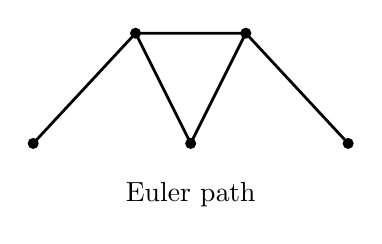
\begin{tikzpicture}[line width=1pt]
\coordinate (a) at (-2,0); \coordinate (b) at (-.7,1.4); \coordinate (c) at (.7,1.4); \coordinate (d) at (2,0);
\draw (a)--(b)--(c)--(d) (b)--(.0,0)--(c);
\foreach \p in {a,b,c,d} \fill (\p) circle (2pt); \fill (0,0) circle (2pt);
\node at (0,-.65) {Euler path};
\end{tikzpicture}
\end{document}
